\documentclass{assignment}

\class{SI 315}
\title{Assignment 1}
\author{Silas Falde}

\begin{document}
\maketitle
\tableofcontents

\section{Network 1}
\begin{figure}[h]
    \centering
    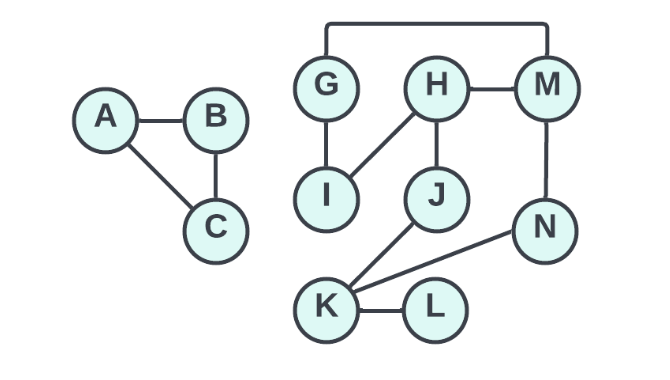
\includegraphics[width=0.5\textwidth]{figs/network-1.png}
    % List of connections (non-directional): 
    % component 1:
    % a to b, a to c
    % b to c
    % component 2: 
    % G to M, G to I
    % M to H, M to N
    % H to I, H to J
    % J to K
    % K to N
    % K to L
\end{figure}

\subsection{Longest Cycles}
\begin{problem}
Identify the longest cycles in the network.
\end{problem}
The cycle $I \to G \to M \to N \to K \to J \to H \to I$ has 7 nodes and is the only longest cycle.

\subsection{Connectedness}
\begin{problem}
Is the network connected? Explain.
\end{problem}

The network is not connected because there are nodes that cannot be reached from other nodes (e.g. $B \to I$).

\subsection{Connected Components}

\begin{problem}
How many connected components does the network have? Which nodes are in each component?
\end{problem}

The network has two connected components:
\begin{itemize}
    \item Component 1: $A, B, C$
    \item Component 2: $G, M, N, K, L, J, H, I$
\end{itemize}

\subsection{Size of Connected Components}

\begin{problem}
How many nodes are in the largest component of the network?
\end{problem}
The largest component is Component 2, which has 8 nodes: $G, M, N, K, L, J, H, I$.

\subsection{Breadth-First Search}
\begin{problem}
Find the distance from node H to every other node in the network using breadth-first search. Draw a diagram of the breadth-first search procedure similar to the one shown in class, where each new layer of nodes is identified and circled. Remember, the BFS diagram should have all of the nodes in it!
\end{problem}

The breadth-first search layers starting at $H$ are:
\begin{itemize}
    \item Distance $0$: $H$
    \item Distance $1$: $I, J, M$
    \item Distance $2$: $G, K, N$
    \item Distance $3$: $L$
    \item Unreachable from $H$: $A, B, C$
\end{itemize}

% TODO: Draw the BFS diagram for the network starting at node H.

\subsection{Add One Edge}
\begin{problem}
What is the longest cycle you can make by adding one edge to the network? Please specify what edge you would add, how long the longest resulting cycle is, and the cycle itself (i.e., the sequence of nodes). You do not have to explain how you found the edge and the cycle.
\end{problem}

The longest cycle can be made by adding the edge $C \to G$. The resulting longest cycle is $I \to G \to C \to A \to B \to C \to G \to M \to N \to K \to J \to H \to I$, which has 11 nodes.

\section{Network 2}

\begin{problem}
In the network below, the ties (P, X), (P, Y), (Q, X), (Q, Y), (R, V), and (R, Z) are labeled strong (S), while all others are labeled weak (W).
\end{problem}

\begin{figure}[h]
    \centering
    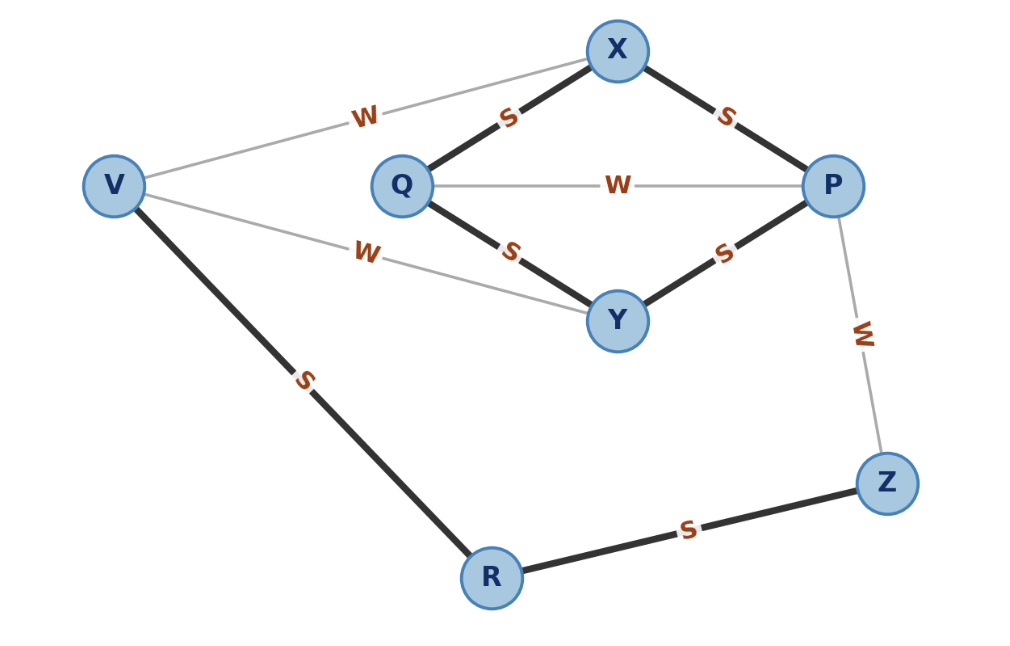
\includegraphics[width=0.8\textwidth]{figs/network-2.png}
    % Strong ties are labeled with (S) and weak ties with (W) in the figure.
    % Connections:
    % P to Q (W), X (S), Y (S), and Z (W)
    % Q to X (S), Y (S)
    % X to V (W)
    % Y to V (W)
    % Z to R (S)
    % V to R (S)
\end{figure}

\subsection{Strong Triadic Closure Property}
\begin{problem}
Identify all nodes that violate the Strong Triadic Closure Property. For each one, name its strong ties and the missing edge.
\end{problem}

The nodes that violate the Strong Triadic Closure Property are $P$, $Q$, and $R$.

\begin{itemize}
    \item $P$ has strong ties to $X$ and $Y$, but $X$ and $Y$ are not adjacent. The missing edge is $XY$.
    \item $Q$ has strong ties to $X$ and $Y$, but $X$ and $Y$ are not adjacent. The missing edge is $XY$.
    \item $R$ has strong ties to $V$ and $Z$, but $V$ and $Z$ are not adjacent. The missing edge is $VZ$.
\end{itemize}

No other node has two strong ties whose endpoints are not connected, so these are the only violations.

\subsection{Fixing the Network}
\begin{problem}
A student says that fixing this network requires the same number of new edges as the number of violations. Is the student right? Explain. Find a smallest set of edges such that adding them makes the network satisfy the Strong Triadic Closure Property. Explain why no smaller set of edges can work.
\end{problem}

The student is wrong because there are 3 violations, but one edge can fix both violations for $P$ and $Q$. The smallest set of edges that fixes all violations is $\{XY, VZ\}$. Adding $XY$ fixes the violations at $P$ and $Q$, and adding $VZ$ fixes the violation at $R$. No smaller set of edges can work because each missing edge corresponds to a distinct violation that cannot be resolved by any other single edge.

\subsection{Local Bridges}
\begin{problem}
List all local bridges in the original network together with their spans. Then list all local bridges again after adding the edges from part (b). Explain why the list changed.
\end{problem}

In the original network, the local bridges are:

\begin{itemize}
    \item $P$--$Z$, span $4$
    \item $Z$--$R$, span $4$
    \item $V$--$R$, span $4$
\end{itemize}

After adding the edges $XY$ and $VZ$, the only local bridge is:

\begin{itemize}
    \item $P$--$Z$, span $3$
\end{itemize}

The list changes because the new edges create triangles and any edge that lies in a triangle cannot be a local bridge, since its endpoints already share a common neighbor.

\subsection{Average Local Clustering Coefficient}
\begin{problem}
Compute the average local clustering coefficient of the network before and after adding the edges identified in part (b). Does the direction of the change match what triadic closure predicts? Explain
\end{problem}

Before adding the edges, the local clustering coefficients are:
\[
    C_P = \frac{2}{6} = \frac{1}{3}, \quad
    C_Q = \frac{2}{3}, \quad
    C_R = 0, \quad
    C_X = \frac{1}{3}, \quad
    C_Y = \frac{1}{3}, \quad
    C_Z = 0, \quad
    C_V = 0.
\]
Thus,
\[
    \overline{C}_{\text{before}} = \frac{1}{7}\left(\frac{1}{3}+\frac{2}{3}+0+\frac{1}{3}+\frac{1}{3}+0+0\right)
    = \frac{5}{21} \approx 0.238.
\]

After adding $XY$ and $VZ$, the local clustering coefficients become
\[
    C_P = \frac{3}{6} = \frac{1}{2}, \quad
    C_Q = 1, \quad
    C_R = 1, \quad
    C_X = \frac{4}{6} = \frac{2}{3}, \quad
    C_Y = \frac{4}{6} = \frac{2}{3}, \quad
    C_Z = \frac{1}{3}, \quad
    C_V = \frac{2}{6} = \frac{1}{3}.
\]
So
\[
    \overline{C}_{\text{after}} = \frac{1}{7}\left(\frac{1}{2}+1+1+\frac{2}{3}+\frac{2}{3}+\frac{1}{3}+\frac{1}{3}\right)
    = \frac{9}{14} \approx 0.643.
\]

The average local clustering coefficient increases from about $0.238$ to about $0.643$. This matches triadic closure: adding edges that complete open triples creates more closed triplets and therefore raises clustering, so the direction of change is exactly what triadic closure predicts.

\section{Network 3}

\subsection{Strong and Weak Ties}
\begin{figure}[h]
    \centering
    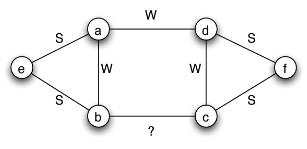
\includegraphics[width=0.5\textwidth]{figs/network-3.png}
    % Network 3 diagram showing strong and weak ties: 
    % E connected to A (S) and B (S)
    % A connected to B (W) and D (W)
    % B connected to C (?)
    % C connected to D (W) and F (S)
    % D connected to F (S)
\end{figure}
\begin{problem}
Consider the graph in which each edge — except the edge connecting b and c — is labeled as a strong tie (S) or a weak tie (W). According to the theory of strong and weak ties, with the strong triadic closure assumption, how would you expect the edge connecting b and c to be labeled? Give a brief (1-3 sentence) explanation for your answer.
\end{problem}

We would expect the edge between $B$ and $C$ to be a weak tie. According to the strong triadic closure assumption, since $B$ has strong ties to $A$ and $E$, the edge connecting $B$ and $C$ should be weak to avoid violating the assumption that strong ties tend to close triangles.

\subsection{Strong Triadic Closure Property}
\begin{figure}[h]
    \centering
    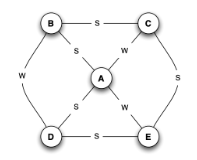
\includegraphics[width=0.5\textwidth]{figs/network-4.png}
    % Network 4 diagram showing strong and weak ties: 
    % A connected to B (S), C (W), D (S), and E(W)
    % B connected to C (S) and D(W)
    % C connected to E (S)
    % D connected to E (S)
\end{figure}
\begin{problem}
In the social network depicted with each edge labeled as either a strong or weak tie, which nodes satisfy the Strong Triadic Closure Property from Chapter 3, and which do not? Provide an explanation for your answer.
\end{problem}

All nodes violate the Strong Triadic Closure Property:
\begin{itemize}
    \item $A$ has strong ties to $B$ and $D$, but $B$ and $D$ are connected only by a weak tie.
    \item $B$ has strong ties to $A$ and $C$, but $A$ and $C$ are connected only by a weak tie.
    \item $C$ has strong ties to $B$ and $E$, but $B$ and $E$ are not connected.
    \item $D$ has strong ties to $A$ and $E$, but $A$ and $E$ are connected only by a weak tie.
    \item $E$ has strong ties to $C$ and $D$, but $C$ and $D$ are not connected.
\end{itemize}

\section{Network 4}
\begin{problem}
Consider an undirected graph with 10 nodes. If the graph has exactly one
local bridge (A,B), is it possible for the graph to also satisfy each of the following
properties? If it's possible, draw a network and explain how it satisfies the properties. If it
is not possible, explain why it is impossible to satisfy all properties.

\textit{Note: You aren't trying to satisfy properties a-d at the same time, but satisfy each, one at
    a time--e.g., if you think part (a) is possible, you'll need to draw a simple, undirected
    graph with 10 nodes that has one edge labeled (A,B) that is a local bridge and also a
    bridge and no other edges that are local bridges; and you need to show that the network
    satisfies all of these conditions.}

% You can draw your network diagrams for each property here using TikZ or include graphics, or with a .dot file.
\end{problem}

\subsection{Edge (A, B) is also a bridge}
This is possible. Use the ten vertices
\[
    \{A,x_1,x_2,x_3,x_4,B,y_1,y_2,y_3,y_4\}.
\]
Make $\{A,x_1,x_2,x_3,x_4\}$ a clique, make
$\{B,y_1,y_2,y_3,y_4\}$ a clique, and add the edge $AB$.
The edge $AB$ is a bridge because removing it separates the two cliques.
It is also the only local bridge: every edge inside either clique is in a
triangle, while $AB$ has no common neighbor.

\begin{figure}[h]
    \centering
    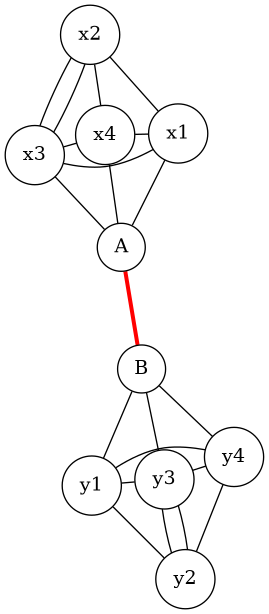
\includegraphics[width=0.3\textwidth]{figs/network-4a.png}
    \caption{Network for part (a). The red edge is $AB$.}
\end{figure}

\subsection{Edge (A, B) has span 4}
This is possible. Arrange the vertices in layers
\[
    L_0=\{A\},\quad L_1=\{c_1,c_2\},\quad
    L_2=\{d_1,d_2\},\quad L_3=\{e_1,e_2\},
    \quad L_4=\{f_1,f_2\},\quad L_5=\{B\}.
\]
Add every edge within a layer, every edge between consecutive layers, and
the edge $AB$. Thus, for example, both $c_1$ and $c_2$ connect to $A$,
both vertices in $L_1$ connect to both vertices in $L_2$, and both vertices
in $L_4$ connect to $B$.

There is a shortest alternate path
\[
    A-c_i-d_j-e_k-f_\ell-B
\]
of length $5$, so $AB$ has span $5-1=4$. The edge $AB$ has no common
neighbor. Every other edge is in a triangle, so $AB$ is the only local
bridge.

\begin{figure}[h]
    \centering
    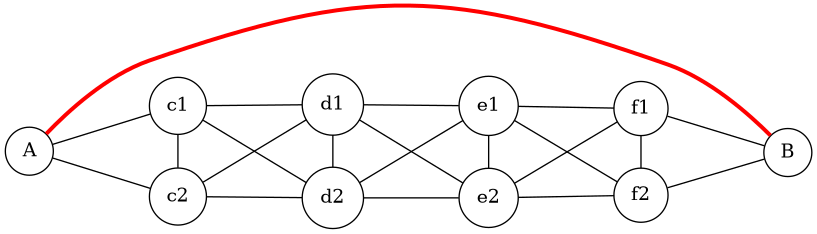
\includegraphics[width=0.7\textwidth]{figs/network-4bc.png}
    \caption{Network for part (b). The red edge is $AB$.}
\end{figure}

\subsection{Nodes A and B both have a local clustering coefficient greater than 0}
This is possible; the layered network described in the previous part works.
The neighbors $c_1,c_2$ of $A$ are adjacent, and the neighbors $f_1,f_2$
of $B$ are adjacent. So both $A$ and $B$ have positive local
clustering coefficients. As above, $AB$ is the only local bridge.

\begin{figure}[h]
    \centering
    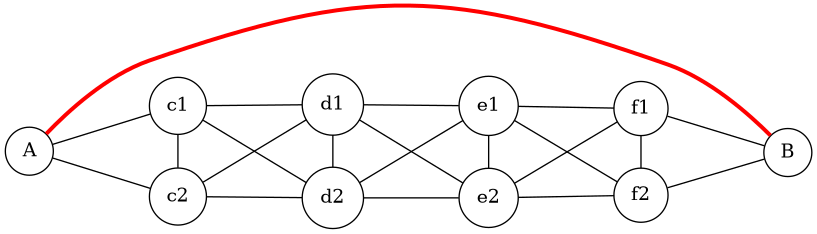
\includegraphics[width=0.7\textwidth]{figs/network-4bc.png}
    \caption{Network for part (c). The red edge is $AB$.}
\end{figure}

\subsection{Edge (A, B) has an embeddedness of 2}
This is impossible. The embeddedness of an edge is the number of common
neighbors of its endpoints. Since $AB$ is a local bridge, $A$ and $B$ have
no common neighbors, so the embeddedness of $AB$ must be $0$, not $2$.4

\section{Network 5}

\begin{problem}
Consider an undirected, connected graph with $n > 2$ nodes. If a node has a local clustering coefficient (LCC) of 0, prove that every edge connected to that node is a local bridge.

\textit{Hint: Think about the definitions: a local bridge is an edge whose removal increases the shortest distance between its endpoints from 1 to at least 3, and a node's LCC = 0 means none of its neighbors are connected. Try proving the statement by contradiction using these ideas.}
\end{problem}

If $v$ is a node with LCC $0$, and $vw$ is any edge connected to
$v$. If $vw$ is \textbf{not} a local bridge, then,
after removing $vw$, there must still be a path from $v$ to $w$ of length
$2$ (or less).

The path cannot have length $1$, because the edge $vw$ was removed. A path
of length $2$ would have the form $v-x-w$. But then $x$ is a neighbor of
$v$ and $w$ is also a neighbor of $v$, and the edge $xw$ connects two
neighbors of $v$. This contradicts LCC$(v)=0$, which says that none of the
neighbors of $v$ are connected to one another. So removing $vw$ disconnects $v$ and $w$ to a distance of at least $3$, which means $vw$ is a local bridge. This applies to any edge connected to $v$.

\end{document}